\documentclass[UTF8,12pt,a4paper]{ctexart}

\usepackage[a4paper,margin=2.4cm]{geometry}
\usepackage{amsmath,amssymb,bm}
\usepackage{graphicx}
\usepackage{booktabs}
\usepackage{longtable}
\usepackage{float}
\usepackage{subcaption}
\usepackage{xcolor}
\usepackage{hyperref}
\usepackage{listings}
\usepackage{enumitem}

\graphicspath{{figures/}{../figures/}}
\hypersetup{colorlinks=true,linkcolor=blue!55!black,urlcolor=blue!55!black,citecolor=blue!55!black}
\setlength{\parindent}{2em}
\setlength{\parskip}{0.25em}
\renewcommand{\arraystretch}{1.18}

\definecolor{codebg}{RGB}{247,247,247}
\definecolor{codeblue}{RGB}{24,95,165}
\definecolor{codegreen}{RGB}{15,110,86}
\lstset{
  language=Python,
  basicstyle=\ttfamily\small,
  keywordstyle=\color{codeblue},
  commentstyle=\color{codegreen},
  stringstyle=\color{red!60!black},
  backgroundcolor=\color{codebg},
  frame=single,
  breaklines=true,
  showstringspaces=false,
  numbers=left,
  numberstyle=\tiny\color{gray},
  xleftmargin=1.5em,
  framexleftmargin=1.2em
}

\title{LUCJ--SQD 中 \texttt{ccsd\_scale} 的作用\\
\large 从截断误差假设到覆盖饱和与概率节点}
\author{Tencent Sparking Program 2026：Problem 2 Optional Problem 1}
\date{2026年7月}

\begin{document}
\maketitle

\begin{abstract}
Problem 2 的 Optional Problem 1 提出：增大 CCSD 振幅缩放参数 \texttt{ccsd\_scale}（记为 $\lambda$）一方面可以使 LUCJ 态偏离 Hartree--Fock（HF）态，提高相关组态的采样覆盖；另一方面会放大 local LUCJ 相对完整 UCJ 的截断误差，因此预期 SQD 能量随 $\lambda$ 先改善、后恶化，并存在内部最优值。

本文对这一预期进行了系统检验。我们使用 PySCF 计算分子积分、CCSD 振幅和 FCI 参考能量，使用 ffsim 构造 local/full UCJ 态并采样，使用 Qiskit Addon SQD 进行采样子空间对角化，并使用 Qiskit Aer 测试门级噪声。实验调节了分子、键长、采样数、噪声、LUCJ 层数和 $\lambda$ 范围。常规参数扫描没有发现稳定、宽广的能量回升区间。进一步的受控实验表明：题目所说的截断误差首先体现为 local LUCJ 与 full UCJ 的态和概率分布差异，它会显著影响直接变分能量；但 SQD 不使用输入态的原始振幅，而是在采样到的行列式子空间内重新对角化，因此只要关键组态仍能进入子空间，SQD 对振幅误差具有较强鲁棒性。

最终得到的 SQD 图景不是宽而平滑的 U 型曲线，而是：小 $\lambda$ 时关键组态覆盖不足，误差随 $\lambda$ 增大而下降；覆盖充分后误差接近由可达支持集决定的平台；在极大 $\lambda$ 的离散概率节点附近，关键组态概率接近零，有限采样会产生窄尖峰。实践中合理的选择不是寻找一个普适的内部最优 $\lambda$，而是选择刚刚进入覆盖饱和区的最小 $\lambda$。
\end{abstract}

\tableofcontents
\newpage

\section{研究动机}

\subsection{Optional Problem 1 的预期}

LUCJ 采样态由 CCSD 振幅构造。引入缩放参数 $\lambda$ 后，$\lambda=0$ 对应 HF 极限，增大 $\lambda$ 会提高激发组态的权重。题目同时指出，local LUCJ 只保留部分局域、相邻的密度--密度耦合，未保留的非相邻项会造成截断误差，并给出其随 $\lambda^2$ 增长的定性描述。

据此，一个自然猜想是：
\begin{enumerate}[label=(\arabic*)]
  \item 小 $\lambda$：采样态过于接近 HF，相关组态覆盖不足，SQD 误差较大；
  \item 中等 $\lambda$：覆盖改善占优，SQD 误差下降；
  \item 大 $\lambda$：local 截断误差占优，SQD 误差重新上升；
  \item 因而存在一个内部最优 $\lambda$。
\end{enumerate}

\subsection{初步结果与疑问}

我们首先按这一思路扫描 $\lambda$，但在 H$_2$、LiH、H$_2$O、N$_2$ 等体系以及不同 shots、键长和噪声设置下，SQD 误差的主要趋势都是下降或饱和，没有出现稳定、宽广、可复现的回升区间。只有在极端 $\lambda$ 和有限采样下出现过孤立尖峰。

这引出两个核心问题：
\begin{itemize}
  \item 题目中的“截断误差”究竟对应什么物理量？
  \item 即使 local 截断显著影响输入量子态，它是否必然以同样方式影响 SQD 能量？
\end{itemize}

本文不预设 U 型趋势必然存在，而是通过参数扫描、受控对照和理论分析，确定 $\lambda$ 真正影响 SQD 的路径。

\section{计算方法与实验设置}

\subsection{软件与基本流程}

计算流程如下：
\begin{enumerate}
  \item \textbf{PySCF}：RHF、活性空间积分、CCSD 振幅和 FCI 参考能量；
  \item \textbf{ffsim}：构造 \texttt{UCJOpSpinBalanced}、local/full UCJ 态矢量及有限-shot 采样；
  \item \textbf{Qiskit Addon SQD}：组态恢复和采样子空间对角化；
  \item \textbf{Qiskit Aer}：门级去极化和热弛豫噪声测试。
\end{enumerate}

SQD 使用采到的 Slater 行列式 $\{|D_k\rangle\}$ 张成子空间
\begin{equation}
\mathcal S=\operatorname{span}\{|D_k\rangle\},
\end{equation}
并求解
\begin{equation}
E_{\mathrm{SQD}}(\mathcal S)
=\min_{|\phi\rangle\in\mathcal S}
\langle\phi|\hat H|\phi\rangle.
\label{eq:sqd}
\end{equation}

\subsection{扫描参数}

实验调节了以下变量：
\begin{itemize}
  \item 分子：H$_2$、LiH、H$_2$O、N$_2$，并对 C$_2$H$_4$ 做过相应检查；
  \item shots：10--5000，受控实验进一步扩展至 $10^7$；
  \item 键长：平衡构型及拉伸构型；
  \item 噪声：无噪声、bit flip、读出误差、Aer 门级去极化等；
  \item LUCJ 层数：$n_{\mathrm{reps}}=1$ 与 3；
  \item $\lambda$：常规范围 $[0,0.5]$、扩展范围 $[0,2]$，以及节点研究中的 $[0,1000]$。
\end{itemize}

\subsection{受控实验的必要性}

增大 $\lambda$ 或加入噪声会同时改变输入态振幅、各行列式采样概率、原始唯一比特串数、正确粒子数样本比例、恢复后的行列式集合及最终经典子空间维数。仅比较能量曲线，无法判断改善来自“态更准确”还是“子空间更大”。为此我们设计了：
\begin{enumerate}
  \item 精确态矢量下 local/full UCJ 对照；
  \item 固定最大子空间维数 $K$ 的 oracle 对照；
  \item 不固定 $K$ 的关键组态覆盖饱和实验；
  \item 大范围 $\lambda$ 概率节点和尖峰验证。
\end{enumerate}

\section{初步参数探究}

\subsection{采样次数}

以平衡 LiH 的严格活性空间（4 空间轨道、2 活性电子）为例，shots 为 10--200、$\lambda\le1$ 时，样本几乎只有 HF 行列式，SQD 能量基本停留在 HF。shots 增至 500--1000 后，少量激发行列式开始出现，误差随 $\lambda$ 下降。这里的主要误差不是普通期望值测量误差，而是\textbf{采样子空间不完备误差}；其收敛往往是台阶式的。

\subsection{键长和分子类型}

拉伸键长会增强静态相关，使 HF 与 FCI 的差距增大，因此小 $\lambda$ 区域的覆盖不足更明显。但在 H$_2$、LiH、H$_2$O 和 N$_2$ 的常规扫描中，增大 $\lambda$ 后误差仍主要表现为下降或饱和。

N$_2$ 的残余误差显著较大。这不仅源于空间规模，还包括三键和拉伸构型的强相关、有限 shots 对关键行列式的低覆盖，以及单参考 CCSD 振幅在多参考区域的质量限制。

\subsection{噪声}

在小活性空间中，不受控地加入 bit flip 或去极化噪声有时会使 SQD 更接近 FCI，因为噪声生成额外候选字符串，组态恢复后碰巧补充了缺失行列式。固定子空间预算并进行粒子数后选择后，H$_2$O 的结果如表~\ref{tab:noise}。

\begin{table}[H]
\centering
\caption{H$_2$O，$S=500$、$\lambda=2$ 时的受控噪声结果。}
\label{tab:noise}
\begin{tabular}{lcc}
\toprule
设置 & SQD 误差（mHa） & 合法样本比例 \\
\midrule
无噪声 & 44.03 & 1.000 \\
1\% bit flip & 44.22 & 0.875 \\
5\% bit flip & 45.27 & 0.517 \\
2\% 读出误差 & 44.67 & 0.762 \\
\bottomrule
\end{tabular}
\end{table}

普通噪声没有显示出系统优势；此前“噪声促进收敛”的现象主要来自不受控的候选子空间扩张。

\begin{figure}[H]
\centering
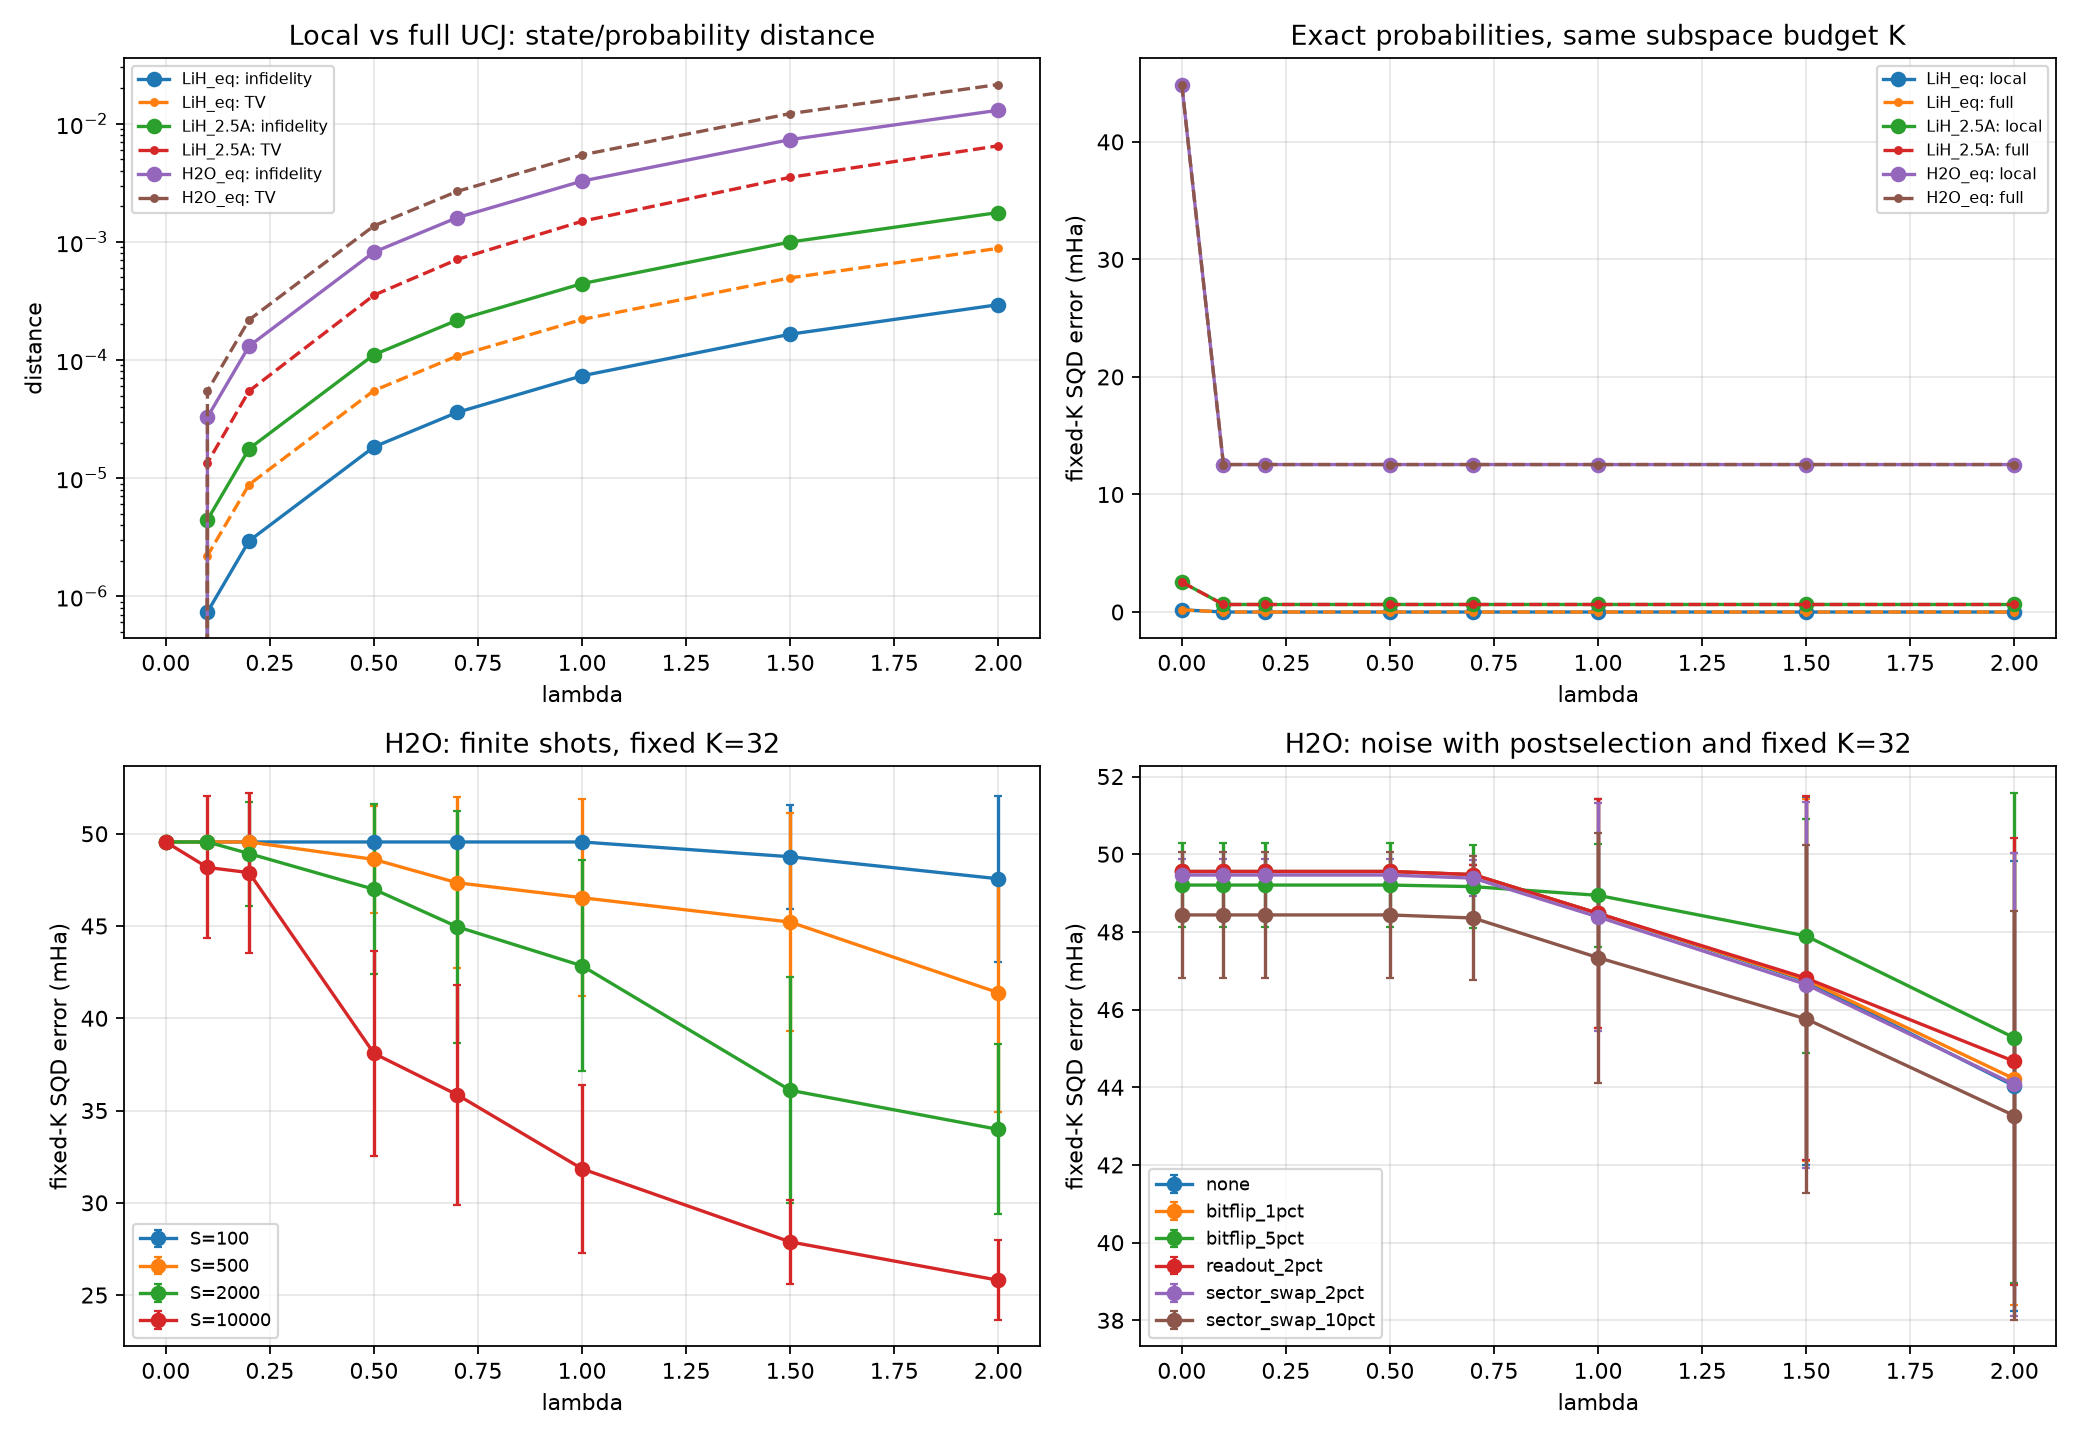
\includegraphics[width=0.96\textwidth]{controlled_experiments.png}
\caption{受控实验汇总。左上：local/full UCJ 态距离；右上：固定 $K$ 的 oracle SQD；左下：H$_2$O 有限-shot 收敛；右下：粒子数后选择和固定预算下的噪声对照。}
\label{fig:controlled}
\end{figure}

\subsection{初步结论}

在常规参数范围内，没有观察到题目预期的宽 U 型 SQD 曲线。误差主要由关键组态覆盖不足控制，增大 $\lambda$ 的覆盖收益尚未被 local 截断效应压过。

\section{理论分析}

\subsection{有限 shots 下的关键组态覆盖}

设关键行列式 $D_i$ 的采样概率为 $p_i(\lambda)$，进行 $S$ 次独立采样后至少出现一次的概率为
\begin{equation}
P_i^{\mathrm{seen}}(\lambda)
=1-[1-p_i(\lambda)]^S
\approx1-e^{-S p_i(\lambda)}.
\label{eq:seen}
\end{equation}

在小 $\lambda$ 区域，典型激发振幅满足
\begin{equation}
c_i(\lambda)=\lambda t_i+O(\lambda^2),
\end{equation}
所以
\begin{equation}
p_i(\lambda)=|c_i(\lambda)|^2
\approx\lambda^2|t_i|^2.
\label{eq:p_lambda}
\end{equation}
当 $S p_i\ll1$ 时，增大 $\lambda$ 会显著提高关键组态召回率，SQD 误差随之下降。

\subsection{覆盖充分后的饱和}

当所有重要行列式均满足 $S p_i\gg1$ 时，漏采概率 $e^{-S p_i}$ 已很小。若不同 $\lambda$ 对应的相关支持集相同，则在采样充分极限下
\begin{equation}
E_{\mathrm{SQD}}(\lambda)
=\lambda_{\min}(H|_{\mathcal S})
\end{equation}
与行列式的原始概率权重无关，因而趋于平台。

若两个采样子空间满足 $\mathcal S_1\subseteq\mathcal S_2$，则由变分原理
\begin{equation}
E_{\mathrm{FCI}}
\le E_{\mathrm{SQD}}(\mathcal S_2)
\le E_{\mathrm{SQD}}(\mathcal S_1).
\label{eq:variational}
\end{equation}
因此，在不限制经典子空间、且新增组态不导致原关键组态丢失时，更广的支持不会提高 SQD 最低本征值。

\subsection{截断误差的准确含义}

local LUCJ 删除了完整 UCJ 中部分非相邻密度--密度耦合，使
\begin{equation}
|\Psi_{\mathrm{LUCJ}}(\lambda)\rangle
\ne |\Psi_{\mathrm{UCJ}}(\lambda)\rangle.
\end{equation}

本文计算的 $O(\lambda^2)$ 量为两态的保真度亏损
\begin{equation}
I_{\mathrm{trunc}}(\lambda)
=1-\left|
\langle\Psi_{\mathrm{LUCJ}}(\lambda)|
\Psi_{\mathrm{UCJ}}(\lambda)\rangle
\right|^2.
\label{eq:infidelity}
\end{equation}
小 $\lambda$ 下，态矢量差为 $O(\lambda)$，故保真度亏损以 $O(\lambda^2)$ 开始。但它不是可直接加到 SQD 能量上的 $C\lambda^2$ 惩罚项。

直接变分能量
\begin{equation}
E_{\mathrm{var}}=\langle\Psi|H|\Psi\rangle
\end{equation}
使用全部振幅和相位，会直接受到截断和过旋转影响；SQD 只使用采到的行列式集合并重新对角化。故更准确的表述是：

\begin{quote}
SQD 对输入态的振幅和相位误差较鲁棒，但不对关键组态支持缺失鲁棒。
\end{quote}

\subsection{\texorpdfstring{极大 $\lambda$ 下的概率节点}{极大 lambda 下的概率节点}}

LUCJ 是幺正、非线性的，行列式振幅不会随 $\lambda$ 永远单调增加，而会在大 $\lambda$ 下呈周期或准周期振荡。若某关键行列式在 $\lambda_0$ 附近满足
\begin{equation}
p_i(\lambda)
\approx a(\lambda-\lambda_0)^2,
\end{equation}
有限 shots 下的危险区域由 $S p_i\lesssim1$ 决定：
\begin{equation}
|\lambda-\lambda_0|
\lesssim\frac{1}{\sqrt{aS}}.
\label{eq:width}
\end{equation}
尖峰宽度约按 $S^{-1/2}$ 缩小。增加 shots 会使尖峰变窄，但不会消除精确零概率节点处的峰顶。

\section{进一步验证实验}

\subsection{精确 local/full UCJ 对照}

$\lambda=0.5$ 时的 local/full 态保真度亏损见表~\ref{tab:infidelity}。

\begin{table}[H]
\centering
\caption{$\lambda=0.5$ 时 local/full UCJ 态保真度亏损。}
\label{tab:infidelity}
\begin{tabular}{lc}
\toprule
体系 & $I_{\mathrm{trunc}}$ \\
\midrule
LiH 平衡构型 & $1.84\times10^{-5}$ \\
LiH，2.5~\AA & $1.11\times10^{-4}$ \\
H$_2$O & $8.20\times10^{-4}$ \\
\bottomrule
\end{tabular}
\end{table}

在题目原始 $\lambda\le0.5$ 区间，local/full 态差异较小，但直接变分能量可以更敏感。例如 H$_2$O、$\lambda=0.5$ 时，local LUCJ 变分误差为 43.614~mHa，full UCJ 为 32.788~mHa，差值约 10.83~mHa。

\subsection{固定子空间预算对照}

使用精确态概率选择概率最高的固定数量行列式，并在相同预算下对角化：
\begin{itemize}
  \item LiH 2.5~\AA、$K=8$：$\lambda\ge0.1$ 后误差约固定为 0.640~mHa；
  \item H$_2$O、$K=32$：$\lambda\ge0.1$ 后误差约固定为 12.55~mHa；
  \item local/full 的固定-$K$ SQD 结果几乎相同。
\end{itemize}
这说明 local/full 主要改变了同一批重要行列式的权重，而没有明显改变 top-$K$ 行列式身份。

\subsection{一层与三层 LUCJ 的支持集上限}

H$_2$O 的 FCI 固定粒子数空间维数为 441。以 FCI 权重最大的 10 个行列式为关键组态：
\begin{itemize}
  \item $n_{\mathrm{reps}}=1$：4 个 top-10 行列式概率严格为零，召回率上限仅 0.60；即使 $10^7$ shots 也不能覆盖充分，支持集 SQD 极限约 12.54~mHa；
  \item $n_{\mathrm{reps}}=3$：所有 top-10 行列式均获得非零概率，支持集召回上限变为 1.0，支持集 SQD 极限降至约 1.08~mHa。
\end{itemize}

\begin{figure}[H]
\centering
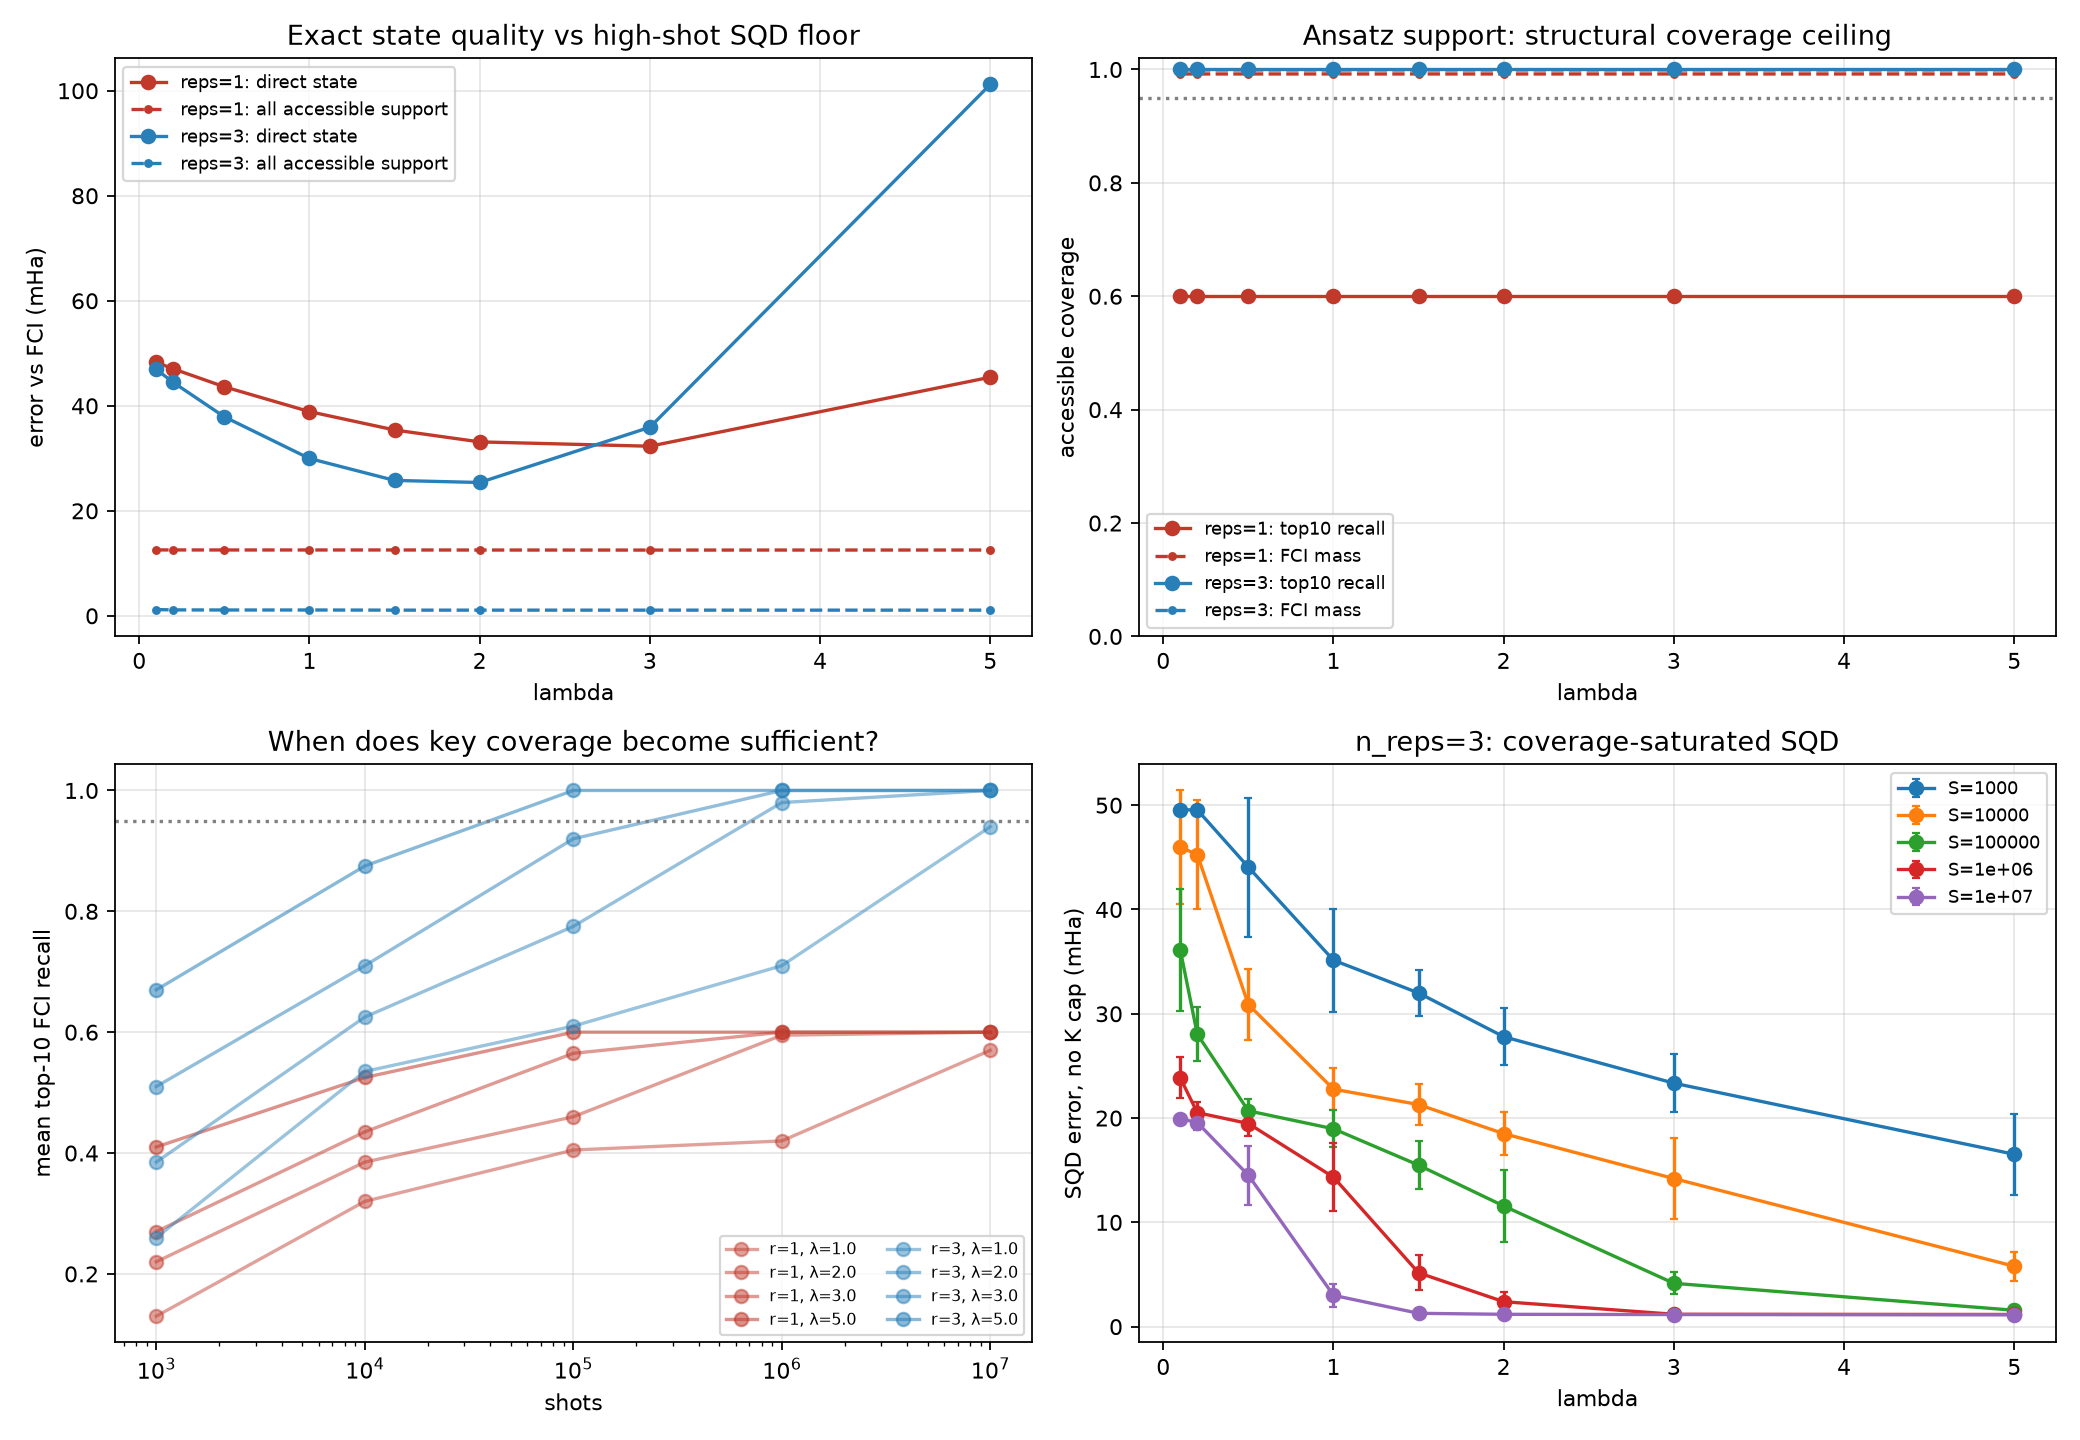
\includegraphics[width=0.96\textwidth]{coverage_saturated.png}
\caption{关键组态覆盖饱和实验。上排比较直接态误差、支持集 SQD 下限和结构性覆盖上限；下排给出召回率随 shots 的增长及不限制 $K$ 的 SQD 曲线。}
\label{fig:saturation}
\end{figure}

\subsection{\texorpdfstring{不限制 $K$ 的覆盖饱和实验}{不限制 K 的覆盖饱和实验}}

H$_2$O、$n_{\mathrm{reps}}=3$、保留所有采到行列式时，结果见表~\ref{tab:saturation}。

\begin{table}[H]
\centering
\caption{H$_2$O 中直接 LUCJ 误差与不限制 $K$ 的 SQD 误差。}
\label{tab:saturation}
\begin{tabular}{ccc}
\toprule
$\lambda$ & 直接 LUCJ 误差（mHa） & SQD 误差（$S=10^7$，mHa） \\
\midrule
1.0 & 29.96 & 3.71 \\
1.5 & 25.79 & 1.28 \\
2.0 & 25.39 & 1.18 \\
3.0 & 35.91 & 1.16 \\
5.0 & 101.20 & 1.13 \\
10.0 & 487.45 & 1.13 \\
\bottomrule
\end{tabular}
\end{table}

$\lambda\ge5$ 后 SQD 变化范围仅约 0.0058~mHa，形成清晰平台；直接态已严重过旋转，但该恶化没有传递为 SQD 回升。

\subsection{\texorpdfstring{H$_2$}{H2} 概率节点：解析与显式采样}

H$_2$ 当前 LUCJ 只在 HF 和一个双激发行列式上有非零概率，因此
\begin{equation}
\mathbb E[\epsilon_{\mathrm{SQD}}]
=p_{\mathrm{HF}}^S\Delta_{\mathrm{HF}}
+p_D^S\Delta_D,
\end{equation}
其中
\begin{equation}
\Delta_{\mathrm{HF}}=20.525\ \mathrm{mHa},
\qquad
\Delta_D=1599.902\ \mathrm{mHa}.
\end{equation}

我们进一步显式调用 ffsim 抽样，对每个采样子空间实际对角化，每点重复 1000 个随机种子。结果见表~\ref{tab:h2sample} 和图~\ref{fig:h2sample}。

\begin{table}[H]
\centering
\caption{H$_2$ 显式有限-shot SQD 与解析期望对照。}
\label{tab:h2sample}
\begin{tabular}{rrrr}
\toprule
$\lambda$ & shots & 显式采样 SQD（mHa） & 解析期望（mHa） \\
\midrule
55.5 & 500 & 1599.902 & 1599.456 \\
55.5 & 5000 & $1598.302\pm1.600$ & 1595.445 \\
166.4 & 500 & 1599.902 & 1599.623 \\
221.9 & 500 & 20.525 & 20.524 \\
221.9 & 5000 & $20.504\pm0.021$ & 20.522 \\
\bottomrule
\end{tabular}
\end{table}

\begin{figure}[H]
\centering
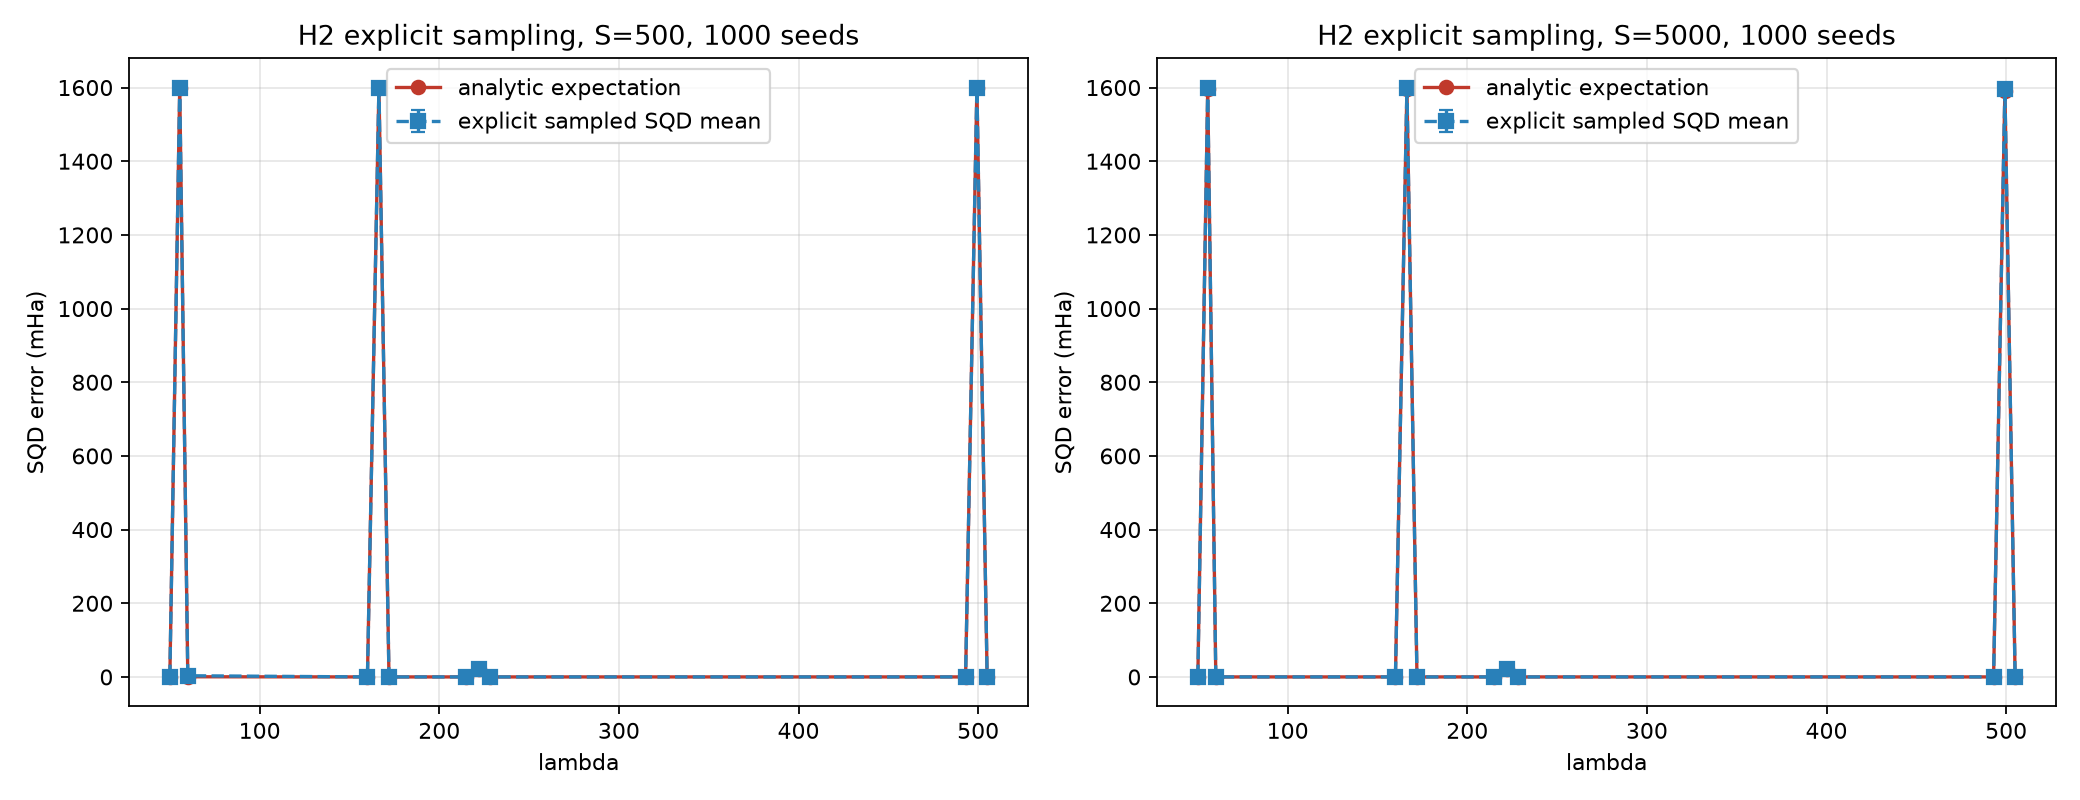
\includegraphics[width=0.92\textwidth]{h2_sampling_validation.png}
\caption{H$_2$ 的解析期望与显式有限-shot SQD 抽样对照。显式采样结果验证了节点尖峰。}
\label{fig:h2sample}
\end{figure}

\subsection{\texorpdfstring{H$_2$O 大范围 $\lambda$ 节点}{H2O 大范围 lambda 节点}}

对 H$_2$O、$n_{\mathrm{reps}}=3$ 在 $\lambda\in[0.1,100]$ 上以 0.05 步长扫描，并连续优化，得到
\begin{equation}
\lambda_0=22.29403997,
\qquad p_{\mathrm{key}}\approx4.0\times10^{-20},
\end{equation}
以及
\begin{equation}
\lambda_0=98.85790158,
\qquad p_{\mathrm{key}}\approx1.44\times10^{-17}.
\end{equation}
节点处 top-10 召回率从 1.0 降至约 0.9，SQD 误差从约 1.12--1.13~mHa 升至约 4.04~mHa。

\begin{table}[H]
\centering
\caption{H$_2$O 关键概率节点的危险窗口全宽。}
\begin{tabular}{lccc}
\toprule
节点 & $S=10^5$ & $S=10^6$ & $S=10^7$ \\
\midrule
$\lambda\approx22.294$ & 0.477 & 0.151 & 0.0477 \\
$\lambda\approx98.858$ & 0.284 & 0.0899 & 0.0284 \\
\bottomrule
\end{tabular}
\end{table}

\begin{figure}[H]
\centering
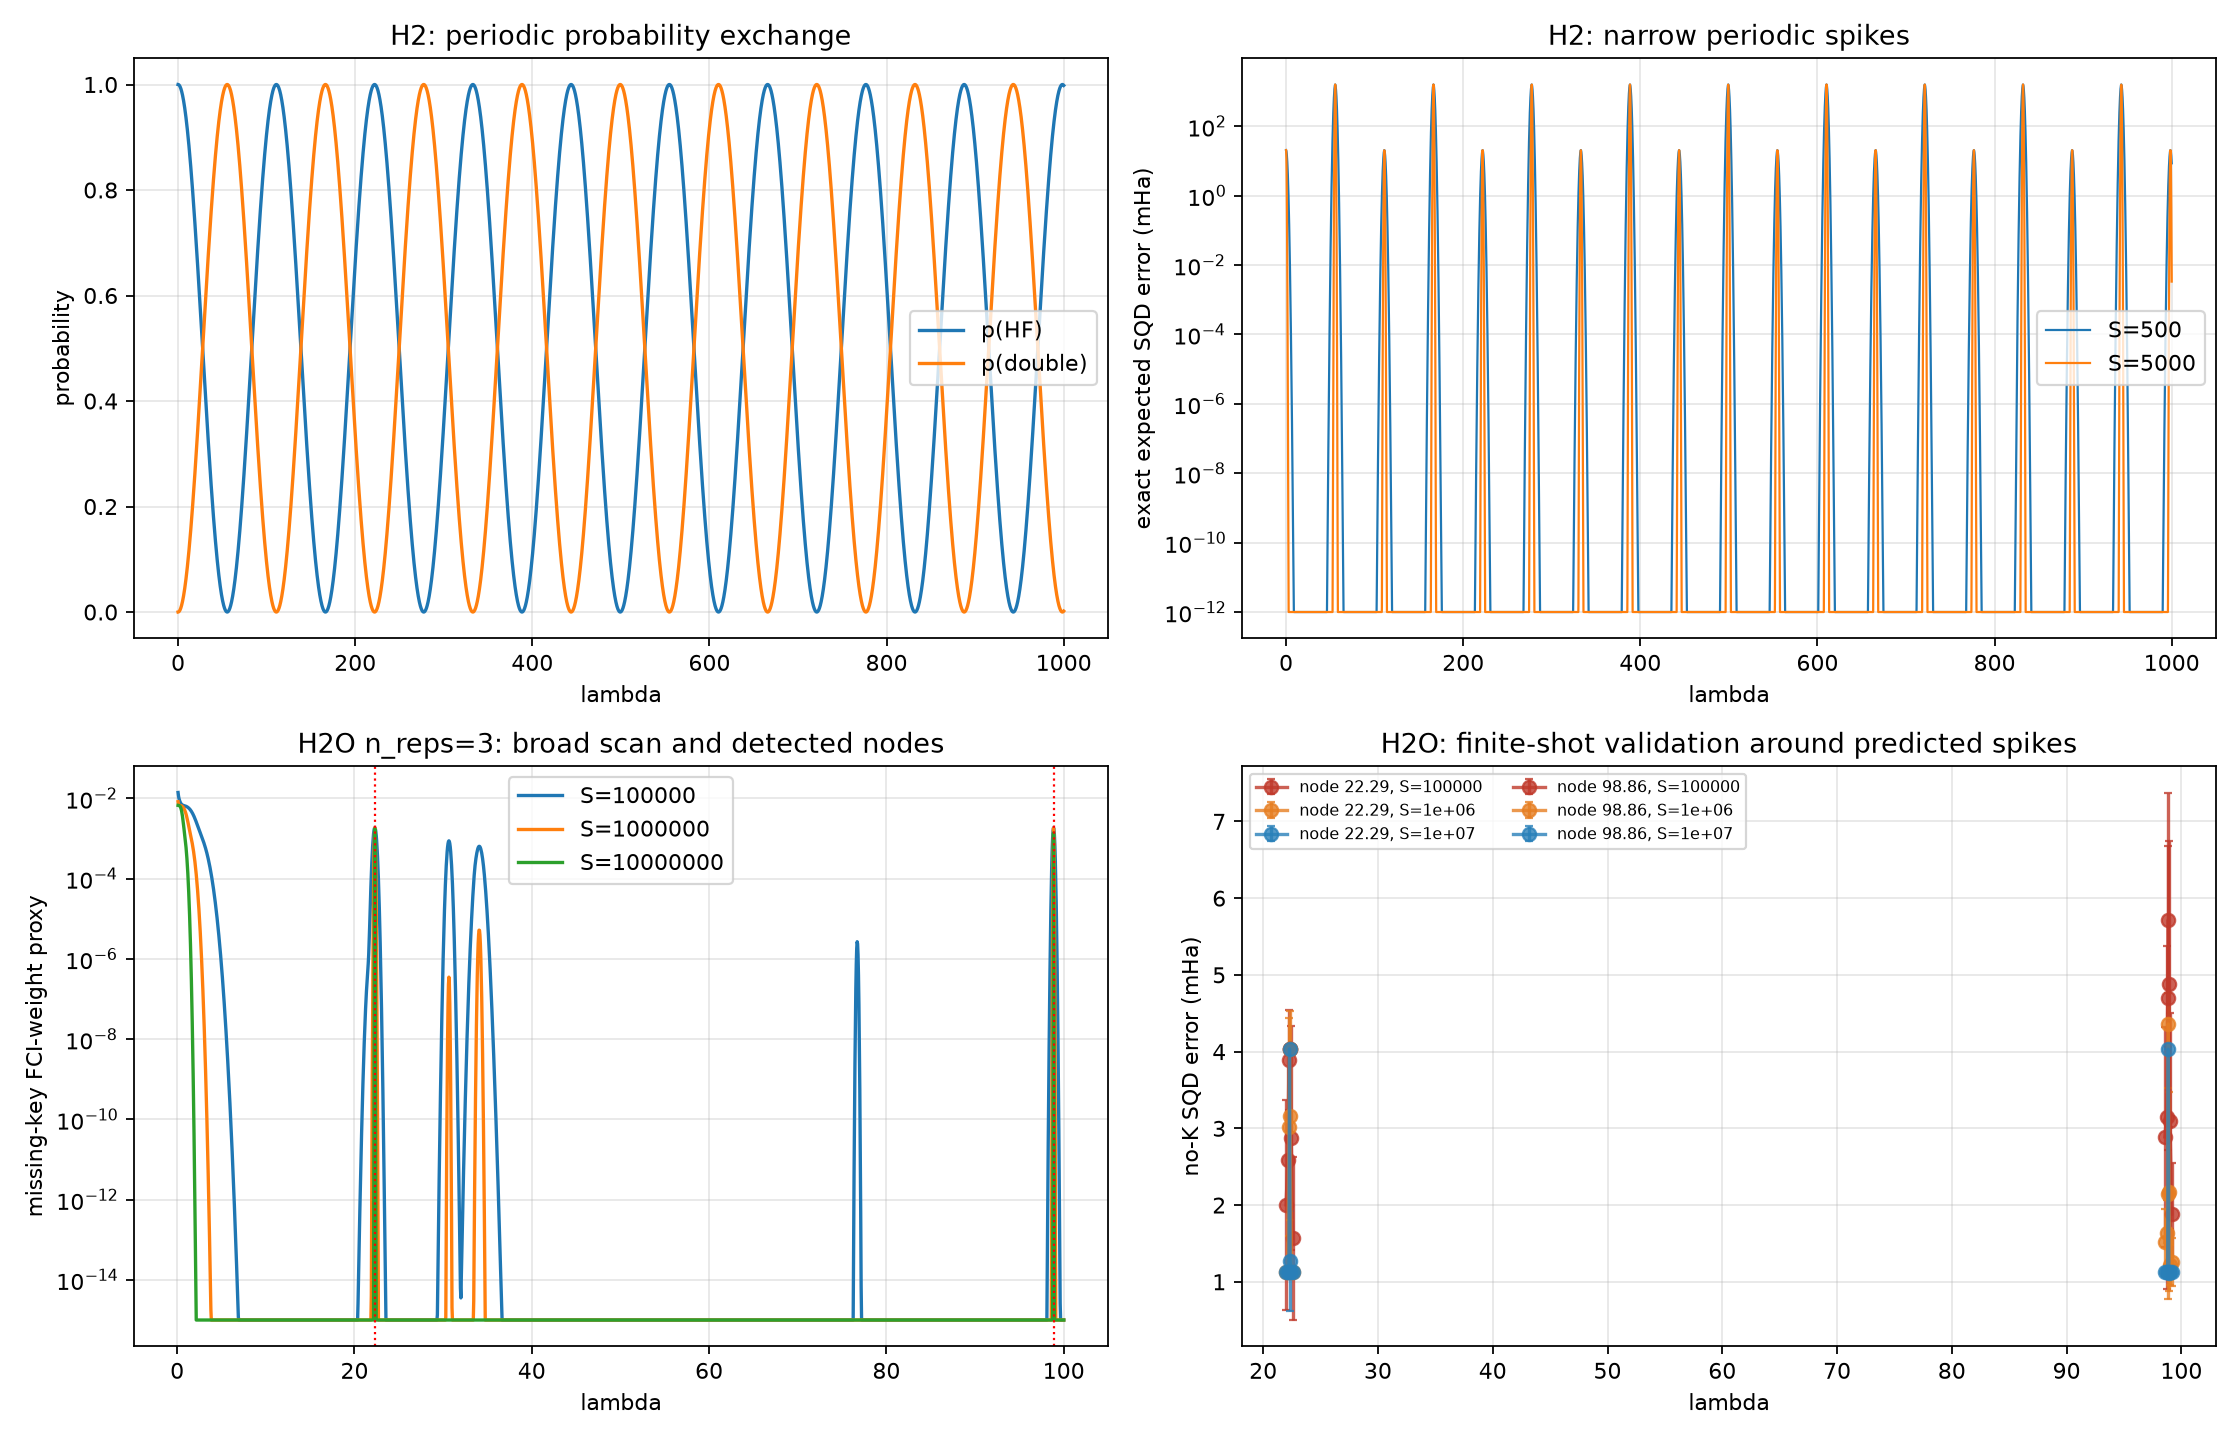
\includegraphics[width=0.98\textwidth]{large_lambda_peaks.png}
\caption{大范围 $\lambda$ 尖峰扫描。上排：H$_2$ 的周期概率交换及精确期望尖峰；下排：H$_2$O 的关键组态遗漏代理量及节点附近显式 SQD 验证。}
\label{fig:peaks}
\end{figure}

\section{讨论}

\subsection{为什么没有出现宽 U 型 SQD 曲线}

题目的直观模型相当于将两个效应写成
\begin{equation}
\epsilon_{\mathrm{SQD}}(\lambda)
\stackrel{?}{=}
\epsilon_{\mathrm{coverage}}(\lambda)+C\lambda^2.
\end{equation}
但实际流程并非如此。$C\lambda^2$ 更接近 local/full 两态距离的标度，而不是直接的 SQD 能量惩罚。SQD 只通过采样集合感受到该差异；若截断改变振幅但不改变关键支持，经典重对角化会消除大部分影响。

当前实验得到的结构是
\begin{equation}
\boxed{
\text{覆盖不足、误差下降}
\ \longrightarrow\ 
\text{关键覆盖饱和平台}
\ +\ 
\text{离散概率节点处的窄尖峰}
}.
\end{equation}

\subsection{\texorpdfstring{实践中的“最佳 $\lambda$”}{实践中的“最佳 lambda”}}

实践中的 $\lambda$ 依赖分子、键长、活性空间、LUCJ 层数、shots、经典子空间预算及噪声条件，不存在普适常数。

在理想、不限制子空间的模型中，平台之后继续增大 $\lambda$ 通常不会显著改善 SQD 能量，却会带来更强过旋转、更多概率节点、更高参数敏感性和更弱物理可解释性。因此可定义覆盖饱和临界 $\lambda_{\mathrm{sat}}$：在给定资源下，选择满足
\begin{equation}
E_{\mathrm{SQD}}(\lambda)-E_{\mathrm{best}}<\delta_E
\end{equation}
且关键组态召回率、有效子空间能量在邻近参数点上稳定的最小 $\lambda$。

\section{结论}

\begin{enumerate}
  \item 初步扫描不支持“local 截断误差随 $\lambda^2$ 平滑增长并最终导致 SQD 能量宽幅回升”的简单图景。
  \item 小 $\lambda$ 时，有限 shots 无法覆盖关键激发行列式；增大 $\lambda$ 提高其采样概率，SQD 误差下降。
  \item 关键组态覆盖充分后，SQD 接近输入态可达支持集决定的下限并进入平台；输入态振幅继续恶化并不必然导致 SQD 回升。
  \item local 截断会显著影响直接变分能量。SQD 对振幅和相位误差较鲁棒，但不对关键组态零概率、有限-shot 漏采和有限预算下的支持缺失鲁棒。
  \item 极大 $\lambda$ 下，幺正概率振荡在离散节点附近产生窄尖峰；尖峰宽度约按 $S^{-1/2}$ 缩小。
  \item 因此，实践中更合理的准则是：在给定 shots、噪声和经典资源下，选择刚刚达到关键组态覆盖饱和的最小 $\lambda$，即饱和临界 $\lambda_{\mathrm{sat}}$。
\end{enumerate}

本问题的主要结论不是寻找由截断误差和覆盖收益平滑平衡得到的普适最优 $\lambda$，而是识别当前资源条件下关键组态覆盖由不足转为饱和的临界 $\lambda$。

\appendix
\section{实验代码清单}

完整实验代码随报告放在 \texttt{code/} 目录中：
\begin{description}
  \item[\texttt{lucj\_sqd\_framework.py}] 分子、LUCJ、采样、噪声与 SQD 的统一框架；
  \item[\texttt{turnaround\_study.py}] 分子、shots、键长、噪声和 $\lambda$ 的参数扫描；
  \item[\texttt{controlled\_optional1\_experiments.py}] 固定 $K$、关键组态覆盖和公平噪声对照；
  \item[\texttt{coverage\_saturated\_experiments.py}] 不限制 $K$ 的覆盖饱和实验；
  \item[\texttt{large\_lambda\_peak\_scan.py}] H$_2$/H$_2$O 大范围节点扫描；
  \item[\texttt{h2\_sampling\_validation.py}] H$_2$ 显式有限-shot SQD 验证。
\end{description}

为避免正文被数百行代码打断，源代码作为独立附件提供。主要入口示例：
\begin{lstlisting}
from lucj_sqd_framework import SQDConfig, LUCJSQDExperiment

cfg = SQDConfig(
    molecule="H2O",
    ccsd_scale=2.0,
    n_reps=3,
    shots=1_000_000,
    noise_model="none",
    config_recovery=True,
)
result = LUCJSQDExperiment(cfg).run()
print(result.summary())
\end{lstlisting}

\section{数据与复现环境}

图中原始数据位于 \texttt{data/}；全部 Python 依赖已打包在 \texttt{environment/sqd\_env/}。建议从项目根目录运行，以保证报告中的相对路径有效。具体方法见根目录 \texttt{README.md}。

\end{document}
